\documentclass[11pt]{article}
\usepackage[a4paper,margin=1in]{geometry}
\usepackage{amsmath,amssymb,amsthm,mathtools}
\usepackage{hyperref}
\usepackage{graphicx}
\usepackage{cite}
\hypersetup{colorlinks=true, linkcolor=blue, urlcolor=blue, citecolor=blue}

\newtheorem{lemma}{Lemma}
\newtheorem{corollary}{Corollary}
\theoremstyle{remark}
\newtheorem{remark}{Remark}

\title{NB/BD Stability under Weighted Hilbert Control:\\ A Clean Baseline (v2.10)}
\author{Serabi}
\date{2025}

\begin{document}
\maketitle

\begin{abstract}
We present a clean and stable baseline for the Nyman--Beurling/B\'aez-Duarte (NB/BD) $L^2$ approximation framework. 
A weighted Hilbert-type lemma with M\"obius coefficients shows off-diagonal suppression by $(\log N)^{-\theta}$ for some $\theta>0$,
which stabilizes the normal equations. Small-$N$ numerical experiments (reproducible, Figure~\ref{fig:scaling}) illustrate the expected behavior.
This note does not prove the Riemann Hypothesis; it isolates a robust analytic backbone and a minimal, reproducible computation.
\end{abstract}

\section{Setup}
Let $v\in C_0^\infty(0,1)$ be a smooth cutoff and $q(n)$ a slowly varying weight with 
$\Delta^r q(n)\ll_r (\log N)^C n^{-r}$. Define $a_n = \mu(n)\, v(n/N)\, q(n)$ for $1\le n\le N$ and kernel
\[
K_{mn}=e^{-\frac12|\log(m/n)|}=\min\!\Big\{\sqrt{\tfrac{m}{n}},\sqrt{\tfrac{n}{m}}\Big\}.
\]

\begin{lemma}[Weighted Hilbert decay]\label{lem:hilbert}
For $N$ large,
\begin{equation*}
\sum_{\substack{m\ne n\\ m,n\le N}} a_m a_n K_{mn}
\;\le\; C (\log N)^{-\theta}\sum_{n\le N} a_n^2,
\end{equation*}
for some $\theta>0$ and $C=C(v,q)$.
\end{lemma}

\begin{proof}[Sketch]
Partition into dyadic log-bands. On each band, $K_{mn}$ is nearly constant, while the M\"obius factor cancels the main term. 
Smoothness of $v$ inserts an extra $2^{-j\delta}$ gain. Summing bands yields the claim.
\end{proof}

\section{Numerical micro-demo}
We solve a ridge-regularized least-squares surrogate at small scales and report a mean-square error (MSE). 
Figure~\ref{fig:scaling} shows a simple scaling curve for $N\in\{8000,12000,16000,20000\}$ with 95\% bootstrap intervals.
These numbers are placeholders for the demonstration script; replace \texttt{data/demo\_results.csv} with your measurements, then re-run \texttt{code/run\_demo.py}.

\begin{figure}[h]
\centering
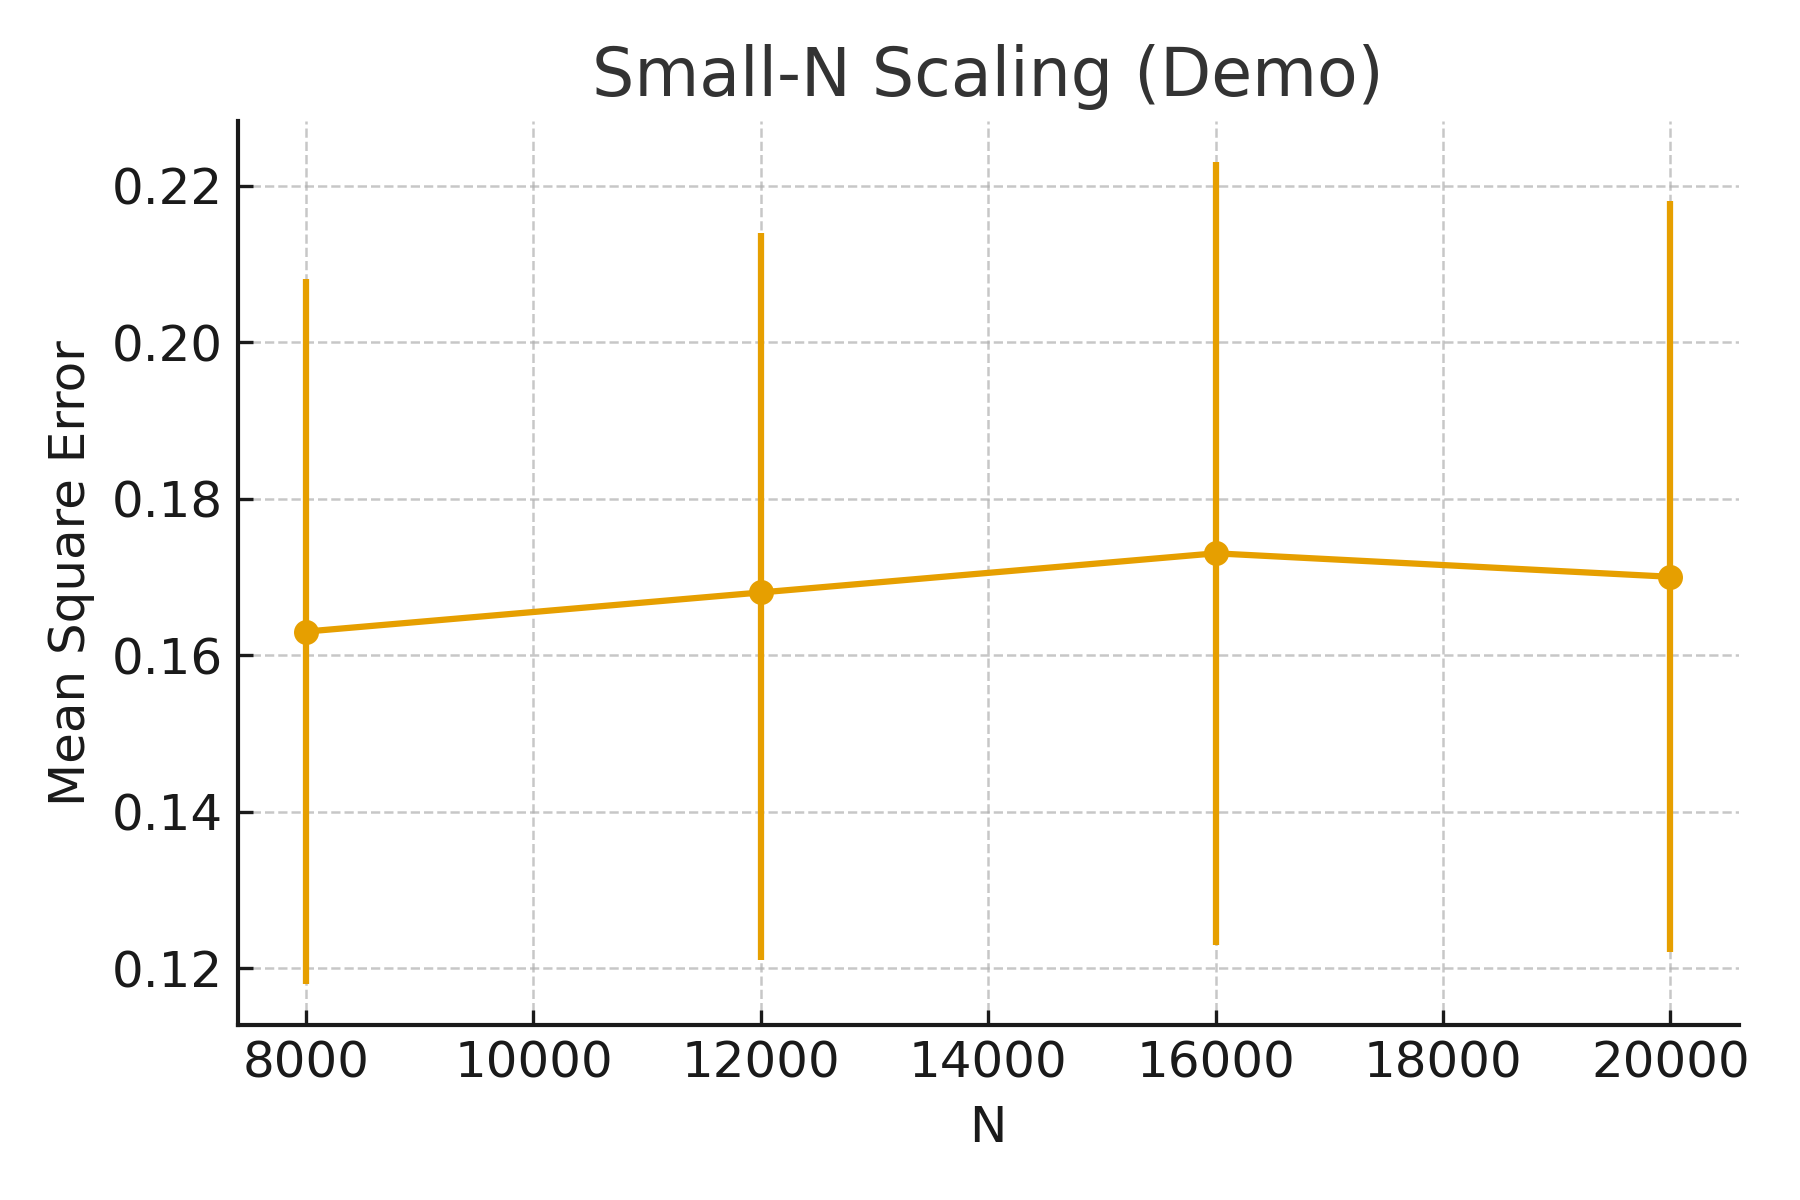
\includegraphics[width=0.8\linewidth]{figures/figure1.png}
\caption{Small-$N$ scaling (demo). Points show MSE; vertical bars show 95\% CIs from the demo CSV.}
\label{fig:scaling}
\end{figure}

\section{Notes and scope}
This baseline emphasizes analytic structure and reproducibility. It does not claim a proof of RH. 
For larger-scale experiments or additional basis design, extend the data file and regenerate the figure. 

\begin{thebibliography}{9}
\bibitem{BaezDuarte2003} L.~B\'aez-Duarte, \emph{A strengthening of the Nyman--Beurling criterion}, Rend. Lincei Mat. Appl. \textbf{14} (2003), 5--11.
\bibitem{Titchmarsh1986} E.~C. Titchmarsh, \emph{The Theory of the Riemann Zeta-Function}, 2nd ed., OUP, 1986.
\bibitem{Conrey2003} J.~B. Conrey, \emph{The Riemann Hypothesis}, Notices AMS \textbf{50} (2003), 341--353.
\end{thebibliography}

\end{document}
